\phantomsection
\section*{Chapter 2}
\addcontentsline{toc}{section}{Chapter 2}

\subsection*{2.4}

\begin{figure}[H]
  \centering
  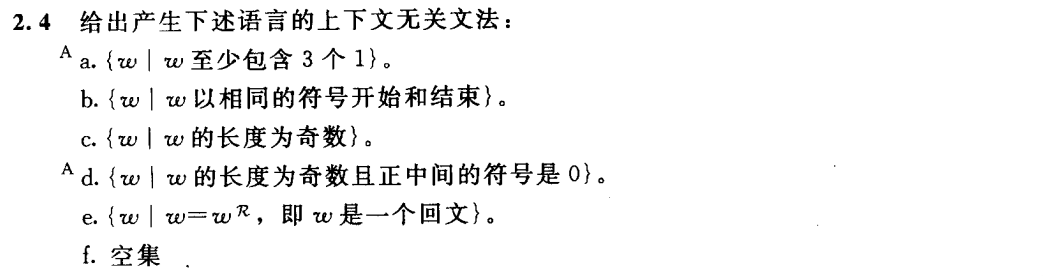
\includegraphics[width=\textwidth]{chapters/imgs/hw_2_4.png}
  \caption{}
  \label{fig:hw_2_4}
\end{figure}

\subsubsection*{解答}

以下各小题默认字母表为 $\Sigma=\{0,1\}$。

\begin{enumerate}[label=(\alph*), leftmargin=2.5em]
    \item 取文法
    \[
        S\to T1T1T1T,
        \qquad
        T\to 0T\mid 1T\mid \varepsilon.
    \]
    其中 $T$ 生成任意二进制串，因此 $S$ 恰好生成至少含有 $3$ 个 $1$ 的字符串。

    \item 取文法
    \[
        S\to 0T0\mid 1T1\mid 0\mid 1,
        \qquad
        T\to 0T\mid 1T\mid \varepsilon.
    \]
    这恰好生成首尾符号相同的所有非空字符串。

    \item 取文法
    \[
        S\to 0E\mid 1E,
    \]
    \[
        E\to 00E\mid 01E\mid 10E\mid 11E\mid \varepsilon.
    \]
    其中 $E$ 生成所有偶长度字符串，因此 $S$ 生成所有奇长度字符串。

    \item 取文法
    \[
        S\to 0
        \mid 0S0
        \mid 0S1
        \mid 1S0
        \mid 1S1.
    \]
    基础情形是中间符号单独为 $0$；每次在左右两侧各添一个任意符号，故长度始终为奇数且中间符号保持为 $0$。

    \item 取文法
    \[
        S\to 0S0\mid 1S1\mid 0\mid 1\mid \varepsilon.
    \]
    这正是回文串的标准上下文无关文法。

    \item 取文法
    \[
        G=(\{S\},\{0,1\},\varnothing,S).
    \]
    即没有任何产生式，因此从开始变量 $S$ 无法推出任何终结符串，故 $L(G)=\varnothing$。
\end{enumerate}

\subsection*{2.6}

\begin{figure}[H]
  \centering
  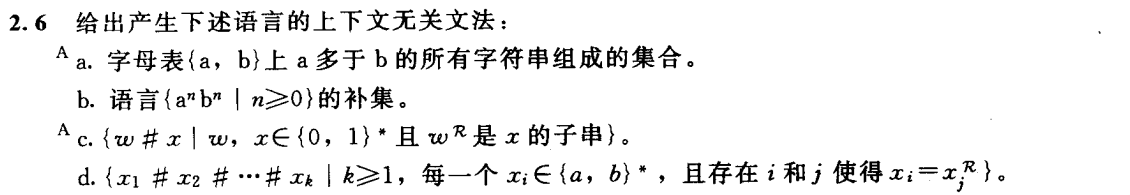
\includegraphics[width=\textwidth]{chapters/imgs/hw_2_6.png}
  \caption{}
  \label{fig:hw_2_6}
\end{figure}

\subsubsection*{解答}

\begin{enumerate}[label=(\alph*), leftmargin=2.5em]
    \item 取文法
    \[
        S\to EaE\mid EaS,
    \]
    \[
        E\to aEbE\mid bEaE\mid \varepsilon.
    \]
    其中 $E$ 生成所有 $a,b$ 个数相同的字符串。于是 $S$ 每次额外保留一个尚未被配平的 $a$，故恰好生成所有 $a$ 的个数多于 $b$ 的字符串。

    \item 这里补集是相对于 $\{a,b\}^*$ 而言。取文法
    \[
        S\to X\mid Y\mid Z,
    \]
    \[
        X\to aXb\mid aA,
        \qquad
        A\to aA\mid \varepsilon,
    \]
    \[
        Y\to aYb\mid B,
        \qquad
        B\to bB\mid b,
    \]
    \[
        Z\to TbaT,
        \qquad
        T\to aT\mid bT\mid \varepsilon.
    \]
    其中 $X$ 生成所有形如 $a^i b^j$ 且 $i>j$ 的串，$Y$ 生成所有形如 $a^i b^j$ 且 $i<j$ 的串，$Z$ 生成所有包含子串 $ba$ 的串，也就是所有不属于 $a^*b^*$ 的串。因此 $S$ 生成的正是
    \[
        \{a,b\}^*\setminus \{a^n b^n\mid n\ge 0\}.
    \]

    \item 取文法
    \[
        S\to RA,
    \]
    \[
        R\to 0R0\mid 1R1\mid \#B,
    \]
    \[
        A\to 0A\mid 1A\mid \varepsilon,
        \qquad
        B\to 0B\mid 1B\mid \varepsilon.
    \]
    其中 $R$ 生成所有形如
    \[
        w\#uw^R
    \]
    的字符串，而 $A$ 再在右侧补上任意后缀。因此 $S$ 恰好生成所有
    \[
        w\#x
        \qquad
        (w^R\text{ 是 }x\text{ 的子串})
    \]
    的字符串。

    \item 设 $T$ 生成任意 $\{a,b\}$-串：
    \[
        T\to aT\mid bT\mid \varepsilon.
    \]
    再令
    \[
        L\to \varepsilon\mid T\#L,
        \qquad
        R\to \varepsilon\mid \#TR,
    \]
    分别生成所选块之前与之后的任意若干块；令
    \[
        M\to T\mid T\#M
    \]
    生成两块之间的任意若干中间块。定义
    \[
        C\to aCa\mid bCb\mid \#\mid \#M\#,
    \]
    则 $C$ 生成形如
    \[
        x\#x^R
        \quad\text{或}\quad
        x\#y_1\#\cdots\#y_m\#x^R
    \]
    的串，即存在两个互为逆序的块。又令
    \[
        P\to aPa\mid bPb\mid a\mid b\mid \varepsilon,
    \]
    它生成所有回文块。于是取开始变量
    \[
        S\to LCR\mid LPR.
    \]
    第一部分 $LCR$ 处理存在 $i\ne j$ 且 $x_i=x_j^R$ 的情形；第二部分 $LPR$ 处理 $i=j$ 时某一块本身就是回文的情形。故该文法生成的正是题目所给语言。
\end{enumerate}

\subsection*{2.8}

\begin{figure}[H]
  \centering
  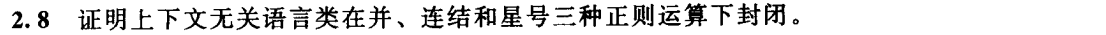
\includegraphics[width=\textwidth]{chapters/imgs/hw_2_8.png}
  \caption{}
  \label{fig:hw_2_8}
\end{figure}

\subsubsection*{证明}

设 $A,B$ 是上下文无关语言。分别取生成它们的上下文无关文法
\[
    G_A=(V_A,\Sigma,R_A,S_A),
    \qquad
    G_B=(V_B,\Sigma,R_B,S_B).
\]
满足
\[
    L(G_A)=A,
    \qquad
    L(G_B)=B.
\]
不妨先把变量重命名，使
\[
    V_A\cap V_B=\varnothing.
\]

\begin{enumerate}[label=(\alph*), leftmargin=2.5em]
    \item 并运算。

    构造新文法
    \[
        G_{\cup}=(V_A\cup V_B\cup\{S\},\Sigma,R,S),
    \]
    其中
    \[
        R=R_A\cup R_B\cup\{S\to S_A\mid S_B\}.
    \]
    从开始变量 $S$ 出发，可先选择导出 $A$ 中的串或 $B$ 中的串，因此
    \[
        L(G_{\cup})=A\cup B.
    \]

    \item 连接运算。

    构造新文法
    \[
        G_{\circ}=(V_A\cup V_B\cup\{S\},\Sigma,R',S),
    \]
    其中
    \[
        R'=R_A\cup R_B\cup\{S\to S_A S_B\}.
    \]
    于是从 $S$ 出发，先导出 $A$ 中某个字符串，再导出 $B$ 中某个字符串，因此
    \[
        L(G_{\circ})=AB.
    \]

    \item 星号运算。

    设
    \[
        G_A=(V,\Sigma,R_A,S_A)
    \]
    满足 $L(G_A)=A$。构造新文法
    \[
        G_*=(V\cup\{S\},\Sigma,R'',S),
    \]
    其中
    \[
        R''=R_A\cup\{S\to \varepsilon\mid S_A S\}.
    \]
    产生式 $S\to\varepsilon$ 对应零次连接，产生式 $S\to S_A S$ 对应先取一个 $A$ 中的串，再继续重复。因此
    \[
        L(G_*)=A^*.
    \]
\end{enumerate}

综上，上下文无关语言类在并、连接与星号运算下封闭。$\blacksquare$

\paragraph{解释.}
这类闭包证明的核心思路是：已知原语言能由 CFG 生成，就直接在 CFG 上做拼装。并运算是在新开始变量处“二选一”；连接运算是让新开始变量先展开成两个旧开始变量；星号运算则是在新开始变量上加入“停止”与“继续接一个块”两种选择。由于这些改动都只引入有限多个新变量和产生式，所得仍是上下文无关文法。

\subsection*{2.10}


\begin{figure}[H]
  \centering
  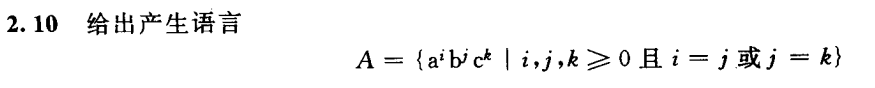
\includegraphics[width=\textwidth]{chapters/imgs/hw_2_10_p1.png}
  \caption{}
  \label{fig:hw_2_10_p1}
\end{figure}

\begin{figure}[H]
  \centering
  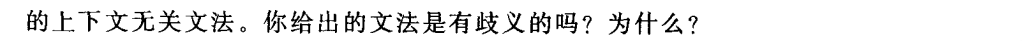
\includegraphics[width=\textwidth]{chapters/imgs/hw_2_10_p2.png}
  \caption{}
  \label{fig:hw_2_10_p2}
\end{figure}

\subsubsection*{解答}

将该语言写成两个较简单语言的并：
\[
    A
    =
    \{a^i b^j c^k\mid i=j\}
    \cup
    \{a^i b^j c^k\mid j=k\}.
\]
也就是
\[
    A
    =
    \{a^n b^n c^k\mid n,k\ge 0\}
    \cup
    \{a^i b^n c^n\mid i,n\ge 0\}.
\]

取文法
\[
    S\to XC\mid AY,
\]
\[
    X\to aXb\mid \varepsilon,
    \qquad
    C\to cC\mid \varepsilon,
\]
\[
    A\to aA\mid \varepsilon,
    \qquad
    Y\to bYc\mid \varepsilon.
\]

其中
\[
    L(X)=\{a^n b^n\mid n\ge 0\},
    \qquad
    L(C)=\{c^k\mid k\ge 0\},
\]
所以
\[
    L(XC)=\{a^n b^n c^k\mid n,k\ge 0\}.
\]
又
\[
    L(A)=\{a^i\mid i\ge 0\},
    \qquad
    L(Y)=\{b^n c^n\mid n\ge 0\},
\]
所以
\[
    L(AY)=\{a^i b^n c^n\mid i,n\ge 0\}.
\]
因此
\[
    L(S)=L(XC)\cup L(AY)=A.
\]

这个文法是有歧义的。原因是
\[
    \{a^n b^n c^n\mid n\ge 0\}\subseteq L(XC)\cap L(AY),
\]
故每个形如 $a^n b^n c^n$ 的字符串都可以从开始变量 $S$ 的两条不同分支导出。以 $abc$ 为例，有两种不同的最左推导：
\[
    S\Rightarrow XC
    \Rightarrow aXbC
    \Rightarrow abC
    \Rightarrow abcC
    \Rightarrow abc,
\]
以及
\[
    S\Rightarrow AY
    \Rightarrow aAY
    \Rightarrow aY
    \Rightarrow abYc
    \Rightarrow abc.
\]
因此该文法是歧义文法。

\begin{figure}[H]
  \centering
  \begin{minipage}[t]{0.47\textwidth}
    \centering
    \[
      S\Rightarrow XC
    \]
    \begin{tikzpicture}[every node/.style={inner sep=1.5pt}]
      \node (S1) at (0,0) {$S$};
      \node (X1) at (-1.4,-1.2) {$X$};
      \node (C1) at (1.4,-1.2) {$C$};

      \node (a1) at (-2.4,-2.4) {$a$};
      \node (X2) at (-1.4,-2.4) {$X$};
      \node (b1) at (-0.4,-2.4) {$b$};

      \node (c1) at (0.8,-2.4) {$c$};
      \node (C2) at (2.0,-2.4) {$C$};

      \node (e1) at (-1.4,-3.5) {$\varepsilon$};
      \node (e2) at (2.0,-3.5) {$\varepsilon$};

      \draw (S1) -- (X1);
      \draw (S1) -- (C1);
      \draw (X1) -- (a1);
      \draw (X1) -- (X2);
      \draw (X1) -- (b1);
      \draw (C1) -- (c1);
      \draw (C1) -- (C2);
      \draw (X2) -- (e1);
      \draw (C2) -- (e2);
    \end{tikzpicture}
  \end{minipage}
  \hfill
  \begin{minipage}[t]{0.47\textwidth}
    \centering
    \[
      S\Rightarrow AY
    \]
    \begin{tikzpicture}[every node/.style={inner sep=1.5pt}]
      \node (S2) at (0,0) {$S$};
      \node (A1) at (-1.3,-1.2) {$A$};
      \node (Y1) at (1.3,-1.2) {$Y$};

      \node (a2) at (-2.0,-2.4) {$a$};
      \node (A2) at (-0.7,-2.4) {$A$};

      \node (b2) at (0.5,-2.4) {$b$};
      \node (Y2) at (1.5,-2.4) {$Y$};
      \node (c2) at (2.5,-2.4) {$c$};

      \node (e3) at (-0.7,-3.5) {$\varepsilon$};
      \node (e4) at (1.5,-3.5) {$\varepsilon$};

      \draw (S2) -- (A1);
      \draw (S2) -- (Y1);
      \draw (A1) -- (a2);
      \draw (A1) -- (A2);
      \draw (Y1) -- (b2);
      \draw (Y1) -- (Y2);
      \draw (Y1) -- (c2);
      \draw (A2) -- (e3);
      \draw (Y2) -- (e4);
    \end{tikzpicture}
  \end{minipage}
  \caption{字符串 $abc$ 对应的两棵不同语法树}
  \label{fig:hw_2_10_parse_trees}
\end{figure}

\paragraph{解释.}
证明一个文法有歧义，只需找出一个字符串 $w\in L(G)$，使它有两棵不同的语法树，或等价地，有两种不同的最左推导（也可用最右推导）。常见做法是先观察文法的不同分支是否会生成重叠的子语言；若文法形如并集拼装
\[
    S\to S_1\mid S_2,
\]
则优先去找
\[
    L(S_1)\cap L(S_2)
\]
中的字符串，因为这样的字符串往往天然会对应两种推导。需要注意的是，证明“这个文法有歧义”只说明当前这套产生式有两种分析方式，并不自动推出该语言本身是固有歧义的；后者要求证明任何文法都会歧义，难度更高。

\subsection*{2.14}

\begin{figure}[H]
  \centering
  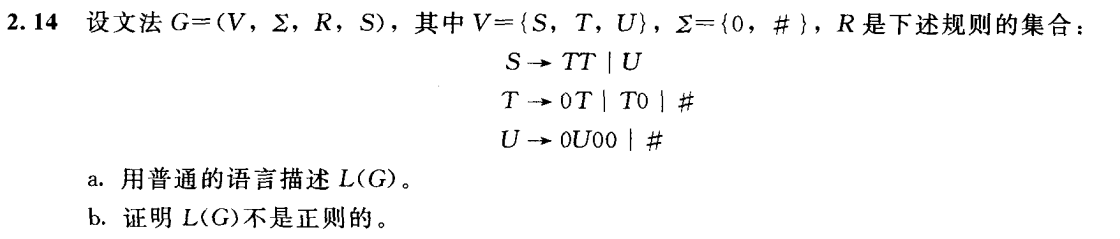
\includegraphics[width=\textwidth]{chapters/imgs/hw_2_14.png}
  \caption{}
  \label{fig:hw_2_14}
\end{figure}

\subsubsection*{解答}

\begin{enumerate}[label=(\alph*), leftmargin=2.5em]
    \item 先分别描述变量 $T,U$ 所生成的语言。

    由
    \[
        T\to 0T\mid T0\mid \#
    \]
    可知，$T$ 最终先变成一个符号 $\#$，随后每用一次产生式 $0T$，就在其左边添一个 $0$；每用一次产生式 $T0$，就在其右边添一个 $0$。因此
    \[
        L(T)=\{0^i\#0^j\mid i,j\ge 0\}.
    \]

    又由
    \[
        U\to 0U00\mid \#
    \]
    可知，$U$ 从 $\#$ 出发，每一步都在左边添一个 $0$，同时在右边添两个 $0$，故
    \[
        L(U)=\{0^n\#0^{2n}\mid n\ge 0\}.
    \]

    于是
    \[
        L(TT)
        =
        \{0^i\#0^j\mid i,j\ge 0\}
        \{0^k\#0^\ell\mid k,\ell\ge 0\}
        =
        \{0^i\#0^m\#0^j\mid i,m,j\ge 0\},
    \]
    因为连接
    \[
        0^i\#0^j\cdot 0^k\#0^\ell
        =
        0^i\#0^{j+k}\#0^\ell.
    \]

    故该文法生成的语言为
    \[
        L(G)
        =
        \{0^i\#0^m\#0^j\mid i,m,j\ge 0\}
        \cup
        \{0^n\#0^{2n}\mid n\ge 0\}.
    \]
    用普通语言描述，即：

    \begin{quote}
        $L(G)$ 由两类字符串组成：一类是恰含两个符号 $\#$、其余位置全为 $0$ 的字符串；另一类是恰含一个符号 $\#$，且其右边 $0$ 的个数恰为左边 $0$ 个数两倍的字符串。
    \end{quote}

    \item 证明 $L(G)$ 不是正则语言。

    取正则语言
    \[
        R=0^*\#0^*.
    \]
    它恰好由所有只含一个符号 $\#$ 的字符串组成。于是
    \[
        L(G)\cap R=\{0^n\#0^{2n}\mid n\ge 0\}.
    \]

    下证
    \[
        K=\{0^n\#0^{2n}\mid n\ge 0\}
    \]
    不是正则语言。若 $K$ 正则，则设其泵长度为 $p$。取
    \[
        s=0^p\#0^{2p}\in K.
    \]
    对任意分解
    \[
        s=xyz,
        \qquad
        |xy|\le p,
        \qquad
        |y|>0,
    \]
    由于前 $p$ 个符号全是 $0$，故必有
    \[
        y=0^t
        \qquad (t>0).
    \]
    令 $i=0$，则
    \[
        xz=0^{p-t}\#0^{2p}.
    \]
    但此时左边 $0$ 的个数为 $p-t$，右边 $0$ 的个数为 $2p$，显然
    \[
        2p\ne 2(p-t),
    \]
    故
    \[
        xz\notin K,
    \]
    与 pumping lemma 矛盾。因此 $K$ 不是正则语言。

    若 $L(G)$ 是正则语言，则因正则语言对交运算封闭，$L(G)\cap R$ 也应正则；但这与上面的结论矛盾。故
    \[
        \boxed{L(G)\text{ 不是正则语言。}}
    \]
\end{enumerate}

\paragraph{解释.}
这题的关键是把文法分成两部分看。变量 $T$ 只是在一个固定的 $\#$ 左右自由添 $0$，所以它生成的是
\[
    0^*\#0^*.
\]
而变量 $U$ 每次递归都“左边加 $1$ 个 $0$、右边加 $2$ 个 $0$”，因此它精确记录了比例关系 $1:2$，生成
\[
    \{0^n\#0^{2n}\mid n\ge 0\}.
\]
证明非正则时，不必直接处理整个并集；只要与正则语言 $0^*\#0^*$ 相交，就能把前一部分滤掉，只剩下后一部分，再对这一部分应用 pumping lemma 即可。

\subsection*{2.16}

\begin{figure}[H]
  \centering
  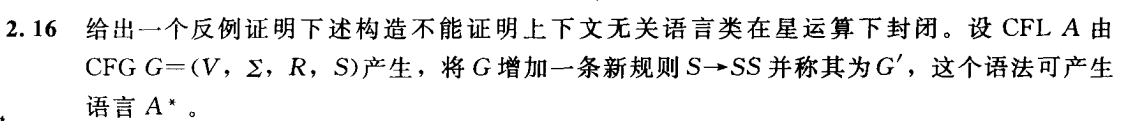
\includegraphics[width=\textwidth]{chapters/imgs/hw_2_16.png}
  \caption{}
  \label{fig:hw_2_16}
\end{figure}

\subsubsection*{解答}

取
\[
    A=\{a\}.
\]
它显然是上下文无关语言。可取文法
\[
    G=(\{S\},\{a\},\{S\to a\},S),
\]
满足
\[
    L(G)=A.
\]

按照题目中的错误构造，在 $G$ 上增加一条规则
\[
    S\to SS,
\]
得到新文法
\[
    G'=(\{S\},\{a\},\{S\to a\mid SS\},S).
\]

这个文法生成的语言是
\[
    L(G')=a^+.
\]
因为每次使用 $S\to SS$ 都会把一个 $a$-块再分成两个非空部分，所以可以生成任意正长度的 $a$ 串；但由于文法中没有推出 $\varepsilon$ 的规则，故
\[
    \varepsilon\notin L(G').
\]

另一方面，
\[
    A^*=\{a\}^*=a^*,
\]
其中必然包含 $\varepsilon$。因此
\[
    L(G')=a^+\ne a^*=A^*.
\]

所以，仅仅给原文法增加一条规则 $S\to SS$，并不能保证得到 $A^*$ 的文法，因而这个构造不能用来证明上下文无关语言类在星号运算下封闭。$\blacksquare$

\paragraph{解释.}
这个构造失败的根本原因是：星号允许取零次连接，因此结果语言必须包含 $\varepsilon$；而在原文法不生成 $\varepsilon$ 时，单加一条 $S\to SS$ 只能实现“重复一次以上”，做不到“零次重复”。正确构造通常要新建一个开始变量，并显式加入
\[
    S_0\to \varepsilon
\]
这一分支。

\subsection*{2.18}

\begin{figure}[H]
  \centering
  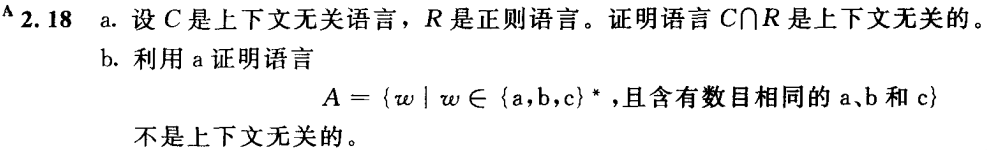
\includegraphics[width=\textwidth]{chapters/imgs/hw_2_28.png}
  \caption{}
  \label{fig:hw_2_28}
\end{figure}

\subsubsection*{证明}

\begin{enumerate}[label=(\alph*), leftmargin=2.5em]
    \item 设 $C$ 是上下文无关语言，$R$ 是正则语言。取识别 $C$ 的 PDA
    \[
        P=(Q_P,\Sigma,\Gamma,\delta_P,q_P,F_P)
    \]
    及识别 $R$ 的 DFA
    \[
        M=(Q_M,\Sigma,\delta_M,q_M,F_M).
    \]

    构造新的 PDA
    \[
        P'=(Q_P\times Q_M,\Sigma,\Gamma,\delta',(q_P,q_M),F_P\times F_M).
    \]
    它的思想是：读入每个符号时，有限控制同时模拟 $P$ 与 $M$；栈操作完全照搬 $P$，而 DFA 的状态只记录在控制状态中。

    按照课本中 PDA 的记法，
    \[
        \delta_P:Q_P\times \Sigma_\varepsilon\times \Gamma_\varepsilon
        \to
        \mathcal{P}(Q_P\times \Gamma_\varepsilon).
    \]
    因此对任意 $p\in Q_P$、$r\in Q_M$、$x\in \Gamma_\varepsilon$，定义 $\delta'$ 如下。

    若 $a\in\Sigma$，则
    \[
        \delta'((p,r),a,x)
        =
        \{((p',\delta_M(r,a)),u)\mid (p',u)\in \delta_P(p,a,x)\}.
    \]
    若进行 $\varepsilon$-转移，则
    \[
        \delta'((p,r),\varepsilon,x)
        =
        \{((p',r),u)\mid (p',u)\in \delta_P(p,\varepsilon,x)\}.
    \]

    也就是说：若
    \[
        (p',u)\in \delta_P(p,a,x),
    \]
    则在 $P'$ 中有
    \[
        ((p',\delta_M(r,a)),u)\in \delta'((p,r),a,x),
    \]
    而若
    \[
        (p',u)\in \delta_P(p,\varepsilon,x),
    \]
    则
    \[
        ((p',r),u)\in \delta'((p,r),\varepsilon,x).
    \]

    于是 $P'$ 在栈上与 $P$ 做完全相同的操作，同时在状态第二分量中记录读入前缀在 DFA $M$ 中所到达的状态。故对任意 $w\in\Sigma^*$，
    \[
        w\in L(P')
        \iff
        w\in C\text{ 且 }w\in R.
    \]
    即
    \[
        L(P')=C\cap R.
    \]
    因此
    \[
        C\cap R
    \]
    是上下文无关语言。$\blacksquare$

    \item 设
    \[
        A=\{w\in\{a,b,c\}^*\mid \#_a(w)=\#_b(w)=\#_c(w)\}.
    \]
    取正则语言
    \[
        R=a^*b^*c^*.
    \]
    则
    \[
        A\cap R=\{a^n b^n c^n\mid n\ge 0\}.
    \]
    这是因为在 $R$ 中，所有 $a$ 都在前，所有 $b$ 居中，所有 $c$ 都在后；再加上三种字母数目相同，就只能得到形如 $a^n b^n c^n$ 的字符串。

    已知
    \[
        \{a^n b^n c^n\mid n\ge 0\}
    \]
    不是上下文无关语言。若 $A$ 是上下文无关语言，则由 (a) 可知 $A\cap R$ 也应是上下文无关语言，这就得到矛盾。故
    \[
        \boxed{
        A=\{w\in\{a,b,c\}^*\mid \#_a(w)=\#_b(w)=\#_c(w)\}
        \text{ 不是上下文无关语言。}}
    \]
\end{enumerate}

\paragraph{解释.}
这题的核心是：正则语言所需的“记忆”是有限的，因此可以直接并入 PDA 的有限控制中；栈仍只负责上下文无关那部分信息。于是 “CFL 条件” 与 “regular 条件” 可以同时检查。第 (b) 问则是反过来用这个封闭性：若一个复杂语言真是 CFL，那么与合适的正则语言相交后也应仍是 CFL；只要把它切出一个已知非 CFL 的子语言，就得到反证。

\subsection*{2.19}

\begin{figure}[H]
  \centering
  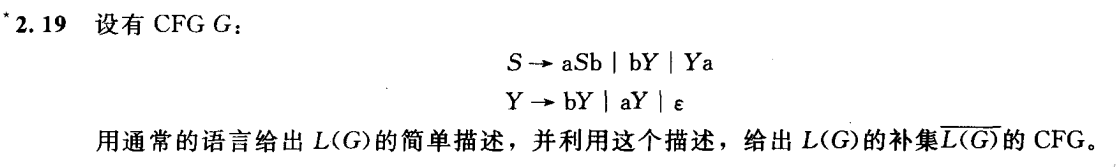
\includegraphics[width=\textwidth]{chapters/imgs/hw_2_19.png}
  \caption{}
  \label{fig:hw_2_19}
\end{figure}

\subsubsection*{解答}

先注意
\[
    Y\to aY\mid bY\mid \varepsilon
\]
生成的正是
\[
    L(Y)=\{a,b\}^*.
\]
因此
\[
    S\to bY
\]
生成所有以 $b$ 开头的字符串，而
\[
    S\to Ya
\]
生成所有以 $a$ 结尾的字符串。规则
\[
    S\to aSb
\]
则是在某个已生成字符串外侧再包上一层首字母 $a$ 和末字母 $b$。

由此可见，$L(G)$ 的简单描述应为
\[
    L(G)=\{a,b\}^*\setminus \{a^n b^n\mid n\ge 0\}.
\]
用通常的语言描述，即：

\begin{quote}
    $L(G)$ 由所有不属于 $\{a^n b^n\mid n\ge 0\}$ 的 $\{a,b\}$-串组成；也就是说，它恰好包含所有不是“先若干个 $a$、再若干个 $b$，且两段长度相等”这种形式的字符串。
\end{quote}

这里并不是“猜”补集，而是先分析补集中字符串被迫具有的结构。设
\[
    C=\{a,b\}^*\setminus L(G).
\]
若 $w\in C$，则：
\begin{enumerate}[label=(\roman*), leftmargin=2.5em]
    \item $w$ 不能以 $b$ 开头；否则由 $S\to bY$ 可得 $w\in L(G)$。
    \item $w$ 不能以 $a$ 结尾；否则由 $S\to Ya$ 可得 $w\in L(G)$。
\end{enumerate}
因此 $w$ 只能是 $\varepsilon$，或可写成
\[
    w=axb
\]
的形式。再者，若 $w=axb\in C$，则必有
\[
    x\in C,
\]
因为一旦 $x\in L(G)$，就可由规则
\[
    S\to aSb
\]
推出 $axb\in L(G)$，矛盾。于是 $C$ 满足递归描述
\[
    C=\{\varepsilon\}\cup aCb.
\]
这已经强制说明：$C$ 中的字符串只能是
\[
    \varepsilon,ab,aabb,aaabbb,\dots,
\]
即
\[
    C\subseteq \{a^n b^n\mid n\ge 0\}.
\]
后面的两步正式证明再进一步说明反向包含也成立，从而得到
\[
    C=\{a^n b^n\mid n\ge 0\}.
\]

下面证明这一点。

\paragraph{先证 $L(G)\subseteq \{a,b\}^*\setminus \{a^n b^n\mid n\ge 0\}$.}
用结构归纳即可。若最外层使用
\[
    S\to bY,
\]
则所得串以 $b$ 开头，不可能属于 $\{a^n b^n\mid n\ge 0\}$；若最外层使用
\[
    S\to Ya,
\]
则所得串以 $a$ 结尾，也不可能属于该集合。若最外层使用
\[
    S\to aSb,
\]
且中间部分 $x\notin \{a^n b^n\mid n\ge 0\}$，则
\[
    axb\notin \{a^n b^n\mid n\ge 0\},
\]
因为若 $axb=a^n b^n$，则必有
\[
    x=a^{n-1}b^{n-1},
\]
矛盾。故一切由该文法生成的字符串都不属于 $\{a^n b^n\mid n\ge 0\}$。

\paragraph{再证反包含.}
对字符串长度作归纳。设
\[
    w\in \{a,b\}^*\setminus \{a^n b^n\mid n\ge 0\}.
\]

若 $w$ 以 $b$ 开头，则由 $S\to bY$ 可得 $w\in L(G)$；若 $w$ 以 $a$ 结尾，则由 $S\to Ya$ 可得 $w\in L(G)$。

剩下的情形是：$w$ 以 $a$ 开头并以 $b$ 结尾。记
\[
    w=axb.
\]
此时 $x$ 仍不属于 $\{a^n b^n\mid n\ge 0\}$；否则若
\[
    x=a^n b^n,
\]
则
\[
    w=a^{n+1}b^{n+1},
\]
与假设矛盾。又因为 $|x|<|w|$，由归纳假设得
\[
    x\in L(G).
\]
于是利用产生式
\[
    S\to aSb
\]
便知
\[
    w=axb\in L(G).
\]

综上，
\[
    L(G)=\{a,b\}^*\setminus \{a^n b^n\mid n\ge 0\}.
\]

因此其补集正是
\[
    \overline{L(G)}=\{a^n b^n\mid n\ge 0\}.
\]
一个识别该补集的 CFG 可以取为
\[
    S_0\to aS_0b\mid \varepsilon.
\]

\paragraph{解释.}
这个文法的两条非递归分支已经覆盖了“以 $b$ 开头”与“以 $a$ 结尾”的所有串；递归分支 $S\to aSb$ 只是在外面再加一层配对的 $a,b$。因此，它恰好漏掉的就是那些既不以 $b$ 开头、也不以 $a$ 结尾、并且不断去掉首尾配对后最终只剩空串的字符串，也就是
\[
    a^n b^n.
\]
一旦看出这一点，补集文法就是标准的
\[
    a^n b^n
\]
文法。

\subsection*{2.22}

\begin{figure}[H]
  \centering
  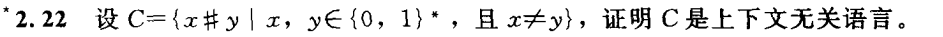
\includegraphics[width=\textwidth]{chapters/imgs/hw_2_22.png}
  \caption{}
  \label{fig:hw_2_22}
\end{figure}

\subsubsection*{证明}

由定理“一个语言是上下文无关语言，当且仅当某个 PDA 识别它”，只需构造一个识别
\[
    C=\{x\#y\mid x,y\in\{0,1\}^*,\ x\ne y\}
\]
的非确定下推自动机即可。

下面给出一个非正式的 PDA 描述。机器在开始时非确定地分成两种情况。

\paragraph{情况 1：检验 $|x|\ne |y|$.}
在读入左半段 $x$ 时，对每个 $0$ 或 $1$ 都向栈中压入一个记号 $X$。读到分隔符 $\#$ 后，开始读入右半段 $y$，每读一个符号就弹出一个 $X$。

\begin{enumerate}[label=(\roman*), leftmargin=2.5em]
    \item 若在 $y$ 尚未读完时栈已空，则说明 $|y|>|x|$，接受。
    \item 若输入已经读完而栈中仍有 $X$，则说明 $|x|>|y|$，接受。
    \item 只有当输入恰好读完且栈也恰好清空时，才说明 $|x|=|y|$，此分支拒绝。
\end{enumerate}

\paragraph{情况 2：检验 $|x|=|y|$ 且某个对应位置符号不同.}
这一分支并不是“猜第一个失配位置”，而只是非确定地猜一个失配见证：若 $x\ne y$，总存在某个对应位置符号不同；机器只要有一条分支猜中这个位置即可。为了便于用栈对齐，我们选择“从右边数的某个失配位置”作为见证。

在读入 $x$ 时，机器在每个位置都有两种转移选择：要么继续向右扫描而什么也不记；要么把当前位置选作待比较位置，并把该符号是 $0$ 还是 $1$ 记在有限控制中。从这以后，每再读入 $x$ 的一个符号，就向栈中压入一个记号 $X$。因此，当读完整个 $x$ 时，栈中记下的正是“该位置右边还剩多少个符号”。

读到 $\#$ 后，机器在 $y$ 中也先通过非确定分支任意跳过一个前缀；随后在某个位置停下，把当前符号作为与前面所记位置对应的比较对象，并要求这个符号与有限控制中记下的符号不同。此后机器继续读完 $y$ 的剩余部分，并对每个剩余符号弹出一个 $X$。只有当输入恰好读完且栈也恰好清空时才接受。

这一条件意味着：在 $x$ 中被选中的位置与在 $y$ 中被选中的位置，右边所剩符号个数相同，也就是说它们是从右边数起的对应位置；而这两个位置上的符号又不同，所以
\[
    x\ne y.
\]

\paragraph{正确性.}
\begin{enumerate}[label=(\roman*), leftmargin=2.5em]
    \item 若 $x\ne y$ 且 $|x|\ne |y|$，则情况 1 接受。
    \item 若 $x\ne y$ 且 $|x|=|y|$，则必存在某个对应位置上的符号不同。取其中任意一个，尤其可取从右边数的某个失配位置。情况 2 总有一条分支能在 $x$ 和 $y$ 中恰好选中这一对位置，于是接受。
    \item 反之，若某分支接受，则要么情况 1 证明了长度不同，要么情况 2 找到了一个从右边数对应、但符号不同的位置，因此一定有 $x\ne y$。
\end{enumerate}

故该 PDA 恰好识别语言 $C$，从而 $C$ 是上下文无关语言。$\blacksquare$

\paragraph{解释.}
你指出的那个问题本质上在于：CFG 很难直接保证“第 $i$ 个位置”对应“第 $i$ 个位置”。而 PDA 用栈天然适合从右往左对齐，所以更自然的做法不是去找“第一次失配”，而是去找“从右边数的某个失配见证”。这里所谓“猜”并不是额外魔法，而正是非确定自动机的标准工作方式：当机器读到某个位置时，它可以沿着多条合法转移同时分支，例如“一条分支把当前位置记为候选失配位置，另一条分支继续向后扫描”。若输入串确实满足 $x\ne y$，那么总存在至少一个真正的失配位置，于是至少有一条分支会恰好选中这个位置并最终验证成功；若输入串不满足条件，则所有分支最终都会失败。

\subsection*{2.24}

\begin{figure}[H]
  \centering
  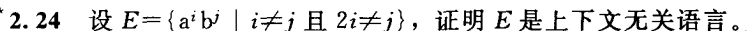
\includegraphics[width=\textwidth]{chapters/imgs/hw_2_24.png}
  \caption{}
  \label{fig:hw_2_24}
\end{figure}

\subsubsection*{证明}

将
\[
    E=\{a^i b^j\mid i\ne j,\ 2i\ne j\}
\]
按 $j$ 与 $i,2i$ 的大小关系拆成三部分：
\[
    E_1=\{a^i b^j\mid j<i\},
\]
\[
    E_2=\{a^i b^j\mid i<j<2i\},
\]
\[
    E_3=\{a^i b^j\mid j>2i\}.
\]
显然
\[
    E=E_1\cup E_2\cup E_3.
\]

下面分别为这三个语言构造 CFG。

\paragraph{情形 $j<i$.}
取文法
\[
    S_1\to aS_1b\mid A,
    \qquad
    A\to aA\mid a.
\]
前一条规则每次同时增加一个 $a$ 和一个 $b$，后一条规则额外产生至少一个未配对的 $a$，故
\[
    L(S_1)=E_1.
\]

\paragraph{情形 $j>2i$.}
取文法
\[
    S_3\to aS_3bb\mid B,
    \qquad
    B\to bB\mid b.
\]
前一条规则每次增加一个 $a$ 和两个 $b$，后一条规则额外产生至少一个未配对的 $b$，故
\[
    L(S_3)=E_3.
\]

\paragraph{情形 $i<j<2i$.}
取文法
\[
    S_2\to aS_2b\mid aTbb,
\]
\[
    T\to aTb\mid aTbb\mid ab.
\]
说明其生成的正是 $E_2$。

若某次推导中，规则
\[
    S_2\to aS_2b
\]
共用了 $m$ 次，然后转入
\[
    S_2\to aTbb,
\]
而在变量 $T$ 中，规则
\[
    T\to aTb
\]
用了 $n$ 次，规则
\[
    T\to aTbb
\]
用了 $t$ 次，最后以
\[
    T\to ab
\]
结束，则最终得到的字符串为
\[
    a^i b^j,
\]
其中
\[
    i=m+n+t+2,
    \qquad
    j=m+n+2t+3.
\]
于是
\[
    j-i=t+1>0,
\]
且
\[
    2i-j=m+n+1>0.
\]
所以
\[
    i<j<2i.
\]
这说明
\[
    L(S_2)\subseteq E_2.
\]

反过来，任取
\[
    a^i b^j\in E_2,
    \qquad i<j<2i.
\]
令
\[
    t=j-i-1\ge 0,
    \qquad
    m=2i-j-1\ge 0.
\]
则
\[
    i=m+t+2,
    \qquad
    j=m+2t+3.
\]
于是让 $S_2\to aS_2b$ 使用 $m$ 次，随后使用一次 $S_2\to aTbb$；再在 $T$ 中使用 $T\to aTbb$ 共 $t$ 次，最后用 $T\to ab$ 收尾，便得到恰好
\[
    a^i b^j.
\]
故
\[
    E_2\subseteq L(S_2).
\]
于是
\[
    L(S_2)=E_2.
\]

最后令
\[
    S\to S_1\mid S_2\mid S_3.
\]
则
\[
    L(S)=E_1\cup E_2\cup E_3=E.
\]
因此 $E$ 是上下文无关语言。$\blacksquare$

\paragraph{解释.}
这题本质上是把平面上所有点 $(i,j)$ 去掉两条直线
\[
    j=i,\qquad j=2i
\]
以后，剩下的区域分成三块：下方、中间、上方。每一块都可以用一个简单 CFG 描述，再用并集拼起来。中间那块
\[
    i<j<2i
\]
稍微麻烦一点，但只要把每个 $a$ 对应产生 $1$ 个或 $2$ 个 $b$，并且强制这两种情况都至少出现一次，就正好落在两条直线之间。

\subsection*{2.26}

\begin{figure}[H]
  \centering
  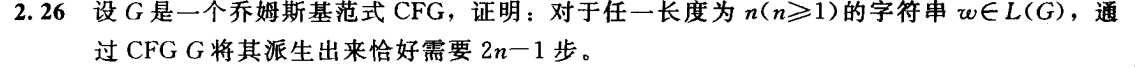
\includegraphics[width=\textwidth]{chapters/imgs/hw_2_26.png}
  \caption{}
  \label{fig:hw_2_26}
\end{figure}

证明。设某个派生
\[
    S\Rightarrow^* w
\]
生成了长度为 $n\ge 1$ 的字符串 $w$。记其中使用形如
\[
    A\to BC
\]
的产生式共 $m$ 次，使用形如
\[
    A\to a
\]
的产生式共 $\ell$ 次。

因为 $G$ 是乔姆斯基范式，且 $w\ne\varepsilon$，所以派生中只能使用这两类产生式。

先求 $\ell$。每次使用 $A\to a$，恰好产生一个终结符；最终得到的字符串长度为 $n$，故
\[
    \ell=n.
\]

再求 $m$。在派生过程中，开始时只有 $1$ 个非终结符 $S$。每次使用
\[
    A\to BC
\]
会使当前非终结符个数增加 $1$；每次使用
\[
    A\to a
\]
会使当前非终结符个数减少 $1$。最终得到终结符串时，非终结符个数为 $0$，因此
\[
    1+m-\ell=0.
\]
代入 $\ell=n$，得
\[
    m=n-1.
\]

故总派生步数为
\[
    m+\ell=(n-1)+n=2n-1.
\]

因此，对任意长度为 $n\ge 1$ 的 $w\in L(G)$，由 $G$ 派生出 $w$ 恰好需要
\[
    2n-1
\]
步。$\blacksquare$

\paragraph{解释.}
这题的关键是：CNF 中只有两种规则。一种把一个非终结符变成两个，因此“未展开的非终结符数”加 $1$；另一种把一个非终结符变成一个终结符，因此这个数减 $1$。终结符一共要产生 $n$ 个，所以第二类规则用了 $n$ 次；从 $1$ 个非终结符降到 $0$ 个，就反推出第一类规则必用 $n-1$ 次。

\subsection*{2.32}

\begin{figure}[H]
  \centering
  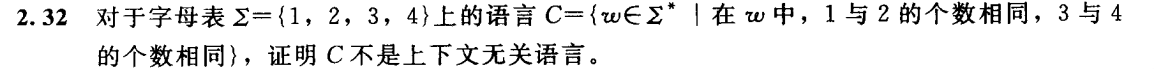
\includegraphics[width=\textwidth]{chapters/imgs/hw_2_32.png}
  \caption{}
  \label{fig:hw_2_32}
\end{figure}

证明。反设
\[
    C=\{w\in\Sigma^*\mid \#_1(w)=\#_2(w),\ \#_3(w)=\#_4(w)\}
\]
是上下文无关语言。由上下文无关语言的泵引理，存在常数 $p$，使得任意满足 $|s|\ge p$ 的 $s\in C$ 都可写成
\[
    s=uvxyz,
\]
其中
\[
    |vxy|\le p,\qquad |vy|>0,
\]
并且对所有 $i\ge 0$，
\[
    uv^i x y^i z\in C.
\]

取
\[
    s=1^p 3^p 2^p 4^p.
\]
显然 $s\in C$，因为
\[
    \#_1(s)=\#_2(s)=p,\qquad \#_3(s)=\#_4(s)=p.
\]

由于每一段
\[
    1^p,\ 3^p,\ 2^p,\ 4^p
\]
的长度都恰为 $p$，而 $|vxy|\le p$，故子串 $vxy$ 至多落在一段中，或至多跨越两段相邻的块。于是只有以下几种情形。

\medskip
\noindent
1. $vxy$ 完全落在某一块中。

若 $vxy$ 落在
\[
    1^p,\ 3^p,\ 2^p,\ 4^p
\]
中的某一块里，则抽引 $i=0$ 或 $i=2$ 只会改变这一类符号的个数，而其对应需要配平的另一类符号个数不变，因此必有
\[
    \#_1\ne \#_2
    \quad\text{或}\quad
    \#_3\ne \#_4.
\]
故所得字符串不在 $C$ 中。

\medskip
\noindent
2. $vxy$ 跨越两段相邻的块。

若跨越
\[
    1^p\text{ 与 }3^p,
\]
则抽引只会改变 $1$ 和 $3$ 的个数，而 $2,4$ 的个数保持为 $p$。由于 $|vy|>0$，至少有一种符号个数发生变化，于是必有
\[
    \#_1\ne \#_2
    \quad\text{或}\quad
    \#_3\ne \#_4.
\]

跨越
\[
    3^p\text{ 与 }2^p
\]
或跨越
\[
    2^p\text{ 与 }4^p
\]
时同理。抽引后，至多只改变两种相邻符号的个数，而至少有一个配平条件被破坏，因此所得字符串也不在 $C$ 中。

\medskip
综上，对任意满足泵引理条件的分解 $s=uvxyz$，总可取 $i=0$ 或 $i=2$ 使得
\[
    uv^i x y^i z\notin C,
\]
与泵引理矛盾。

因此 $C$ 不是上下文无关语言。$\blacksquare$

\paragraph{解释.}
这题和
\[
    \{a^n b^n c^n\mid n\ge 0\}
\]
一样，核心是同时维持两组独立的计数约束。选取
\[
    1^p3^p2^p4^p
\]
以后，泵引理中的短窗口最多只会碰到相邻两块，因此一旦抽引，就不可能同时保持
\[
    \#_1=\#_2,\qquad \#_3=\#_4.
\]

\subsection*{2.33}

\begin{figure}[H]
  \centering
  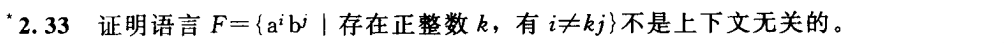
\includegraphics[width=\textwidth]{chapters/imgs/hw_2_33.png}
  \caption{}
  \label{fig:hw_2_33}
\end{figure}

\paragraph{说明.}
按题意，这里应理解为证明
\[
    F=\{a^i b^j\mid i=kj\text{ for some positive integer }k\}
\]
不是上下文无关语言。若写成 $i\ne kj$，则该语言几乎就是整个 $a^*b^*$，命题不成立。

证明。反设 $F$ 是上下文无关语言。由泵引理，存在泵长度 $p$，使得任意满足 $|s|\ge p$ 的 $s\in F$ 都可写成
\[
    s=uvxyz,
\]
其中
\[
    |vxy|\le p,\qquad |vy|>0,
\]
并且对所有 $i\ge 0$，
\[
    uv^i x y^i z\in F.
\]

取素数 $q$，满足
\[
    q>p^2+p.
\]
令
\[
    s=a^{q^2}b^q.
\]
因为
\[
    q^2=q\cdot q,
\]
故 $s\in F$。

对任意满足条件的分解 $s=uvxyz$，记
\[
    \alpha=\#_a(vy),\qquad \beta=\#_b(vy).
\]
则
\[
    0\le \alpha,\beta\le p,\qquad \alpha+\beta>0.
\]

下面分类讨论。

\medskip
\noindent
1. $\beta=0$。

此时 $vy$ 只含字母 $a$。取 $i=0$，得
\[
    uv^0xy^0z=a^{q^2-\alpha}b^q.
\]
因为
\[
    0<\alpha\le p<q,
\]
而 $q\mid q^2$，故
\[
    q\nmid (q^2-\alpha).
\]
因此新的 $a$ 的个数不是 $q$ 的整数倍，从而
\[
    uv^0xy^0z\notin F.
\]

\medskip
\noindent
2. $\alpha=0$。

此时 $vy$ 只含字母 $b$。取 $i=2$，得
\[
    uv^2xy^2z=a^{q^2}b^{q+\beta}.
\]
由于 $q$ 是素数，$q^2$ 的正因子只有
\[
    1,\ q,\ q^2.
\]
而
\[
    q<q+\beta<2q<q^2,
\]
故
\[
    q+\beta\nmid q^2.
\]
因此
\[
    uv^2xy^2z\notin F.
\]

\medskip
\noindent
3. $\alpha>0$ 且 $\beta>0$。

取 $i=2$，得
\[
    uv^2xy^2z=a^{q^2+\alpha}b^{q+\beta}.
\]
若它仍在 $F$ 中，则必须有
\[
    q+\beta\mid q^2+\alpha.
\]
但模 $q+\beta$ 计算，
\[
    q\equiv -\beta \pmod{q+\beta},
\]
故
\[
    q^2+\alpha\equiv \beta^2+\alpha \pmod{q+\beta}.
\]
又因为
\[
    0<\beta^2+\alpha\le p^2+p<q<q+\beta,
\]
所以
\[
    \beta^2+\alpha
\]
是一个严格介于 $0$ 与 $q+\beta$ 之间的余数，不可能为 $0$。因此
\[
    q+\beta\nmid q^2+\alpha,
\]
从而
\[
    uv^2xy^2z\notin F.
\]

\medskip
三种情形都得到矛盾，因此 $F$ 不是上下文无关语言。$\blacksquare$

\paragraph{解释.}
这题的关键不是“比例关系难描述”，而是要找到一个对抽引非常敏感的样本。取
\[
    a^{q^2}b^q
\]
以后，原来的比例恰好是整数倍；但只要把前面的 $a$ 或后面的 $b$ 稍微改动一点，这种整除关系就会立刻失效。选素数 $q$ 的作用，就是让“谁能整除 $q^2$”这件事非常刚性。

\subsection*{2.44}


\begin{figure}[H]
  \centering
  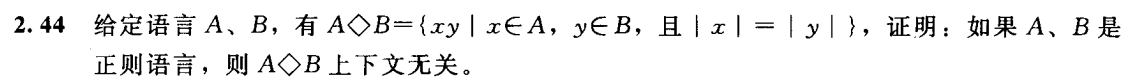
\includegraphics[width=\textwidth]{chapters/imgs/hw_2_44.png}
  \caption{}
  \label{fig:hw_2_44}
\end{figure}

证明。设 $A,B$ 是正则语言。取识别它们的 DFA
\[
    M_A=(Q_A,\Sigma,\delta_A,q_A,F_A),
\]
\[
    M_B=(Q_B,\Sigma,\delta_B,q_B,F_B).
\]

我们构造一台 NPDA 来识别
\[
    A\diamond B=\{xy\mid x\in A,\ y\in B,\ |x|=|y|\}.
\]

这台 NPDA 的思路如下。

\medskip
\noindent
1. 在读入前半段 $x$ 时，它在有限控制中模拟 $M_A$，并且每读入一个符号就向栈中压入一个记号 $X$。

\medskip
\noindent
2. 在某个时刻，它通过一次 $\varepsilon$-转移非确定地猜测：“这里就是分界点，接下来开始读 $y$。”

\medskip
\noindent
3. 在读入后半段 $y$ 时，它在有限控制中模拟 $M_B$，并且每读入一个符号就从栈中弹出一个 $X$。

\medskip
\noindent
4. 当输入恰好读完、栈恰好回到底符号，并且两个 DFA 都处于接受态时，这台 NPDA 接受。

\medskip
形式化地，令栈字母表为
\[
    \Gamma=\{X,\$\},
\]
其中 $\$$ 是栈底符号。状态集取为
\[
    Q=Q_A\times Q_B\times \{1,2\}\ \cup\ \{q_{\mathrm{acc}}\}.
\]
其中第三个分量表示当前处于第一阶段还是第二阶段。开始状态为
\[
    (q_A,q_B,1),
\]
初始栈为 $\$$。

转移规则如下。

\medskip
\noindent
第一阶段：若当前状态为 $(p,r,1)$，读入 $a\in\Sigma$，则转到
\[
    (\delta_A(p,a),r,1),
\]
并向栈中压入一个 $X$。

\medskip
\noindent
阶段切换：对任意 $(p,r,1)$，允许一条 $\varepsilon$-转移到
\[
    (p,r,2),
\]
栈不变。

\medskip
\noindent
第二阶段：若当前状态为 $(p,r,2)$，读入 $a\in\Sigma$，且栈顶为 $X$，则转到
\[
    (p,\delta_B(r,a),2),
\]
并弹出这个 $X$。

\medskip
\noindent
接受：若输入已读完，当前状态为 $(p,r,2)$，其中
\[
    p\in F_A,\qquad r\in F_B,
\]
且栈顶为 $\$$，则通过一条 $\varepsilon$-转移进入接受态 $q_{\mathrm{acc}}$。

\medskip
证明这台 NPDA 识别的正是 $A\diamond B$。

若某串 $w$ 被该 NPDA 接受，则它在某一条接受分支上被分成两段
\[
    w=xy.
\]
第一阶段恰好读完 $x$，故有限控制中的 $M_A$ 模拟表明
\[
    x\in A.
\]
第二阶段恰好读完 $y$，故 $M_B$ 的模拟表明
\[
    y\in B.
\]
又因为第一阶段每读一个符号压入一个 $X$，第二阶段每读一个符号弹出一个 $X$，并且接受时栈恰好回到底符号，所以
\[
    |x|=|y|.
\]
于是
\[
    w\in A\diamond B.
\]

反过来，若
\[
    w=xy\in A\diamond B,
\]
其中
\[
    x\in A,\qquad y\in B,\qquad |x|=|y|,
\]
则这台 NPDA 可以在恰好读完 $x$ 时猜中分界点，随后在第二阶段读入 $y$。由于
\[
    x\in A,\qquad y\in B,
\]
最后两台 DFA 都处于接受态；又因为
\[
    |x|=|y|,
\]
栈中压入与弹出的 $X$ 个数恰好相同，因此最终栈回到底符号，从而接受 $w$。

故
\[
    L(P)=A\diamond B.
\]
因此 $A\diamond B$ 是上下文无关语言。$\blacksquare$

\paragraph{解释.}
这题的本质是把“属于 $A$”“属于 $B$”和“前后两段长度相等”三件事同时检查。前两件事因为 $A,B$ 正则，只需在有限控制中模拟两个 DFA；第三件事则由栈完成，用“前半段压栈、后半段弹栈”的方式记录长度差。非确定性只用来猜分界点。

\subsection*{2.45}

\begin{figure}[H]
  \centering
  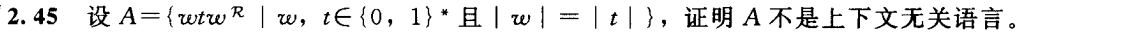
\includegraphics[width=\textwidth]{chapters/imgs/hw_2_45.png}
  \caption{}
  \label{fig:hw_2_45}
\end{figure}

证明。设
\[
    A=\{wtw^R\mid w,t\in\{0,1\}^*,\ |w|=|t|\}.
\]
反设 $A$ 是上下文无关语言。

考虑正则语言
\[
    R=0^*1\,0^*1\,0^*.
\]
由于上下文无关语言对与正则语言求交封闭，故
\[
    L=A\cap R
\]
也应当是上下文无关语言。

下面先刻画 $L$。

若
\[
    s\in A\cap R,
\]
则
\[
    s=wtw^R,\qquad |w|=|t|,
\]
并且 $s$ 恰好含有两个 $1$，其形式为
\[
    0^*1\,0^*1\,0^*.
\]
因此 $t$ 中不能含有 $1$，否则整个串中至少有三个 $1$；同理，$w$ 中也只能含有一个 $1$，否则 $w^R$ 中也会贡献至少两个 $1$，整个串仍会超过两个 $1$。于是必有
\[
    w=0^n1
\]
对某个 $n\ge 0$ 成立。因为
\[
    |w|=n+1=|t|,
\]
而 $t$ 只能由 $0$ 组成，所以
\[
    t=0^{n+1}.
\]
从而
\[
    s=0^n1\,0^{n+1}1\,0^n.
\]

反过来，对任意 $n\ge 0$，
\[
    0^n1\,0^{n+1}1\,0^n
    =(0^n1)\,0^{n+1}\,(0^n1)^R
\]
且
\[
    |0^n1|=n+1=|0^{n+1}|,
\]
故它属于 $A$；又显然属于 $R$。于是
\[
    L=\{0^n1\,0^{n+1}1\,0^n\mid n\ge 0\}.
\]

现在用上下文无关语言的泵引理证明 $L$ 不是上下文无关语言。设 $p$ 是泵长度，取
\[
    s=0^p1\,0^{p+1}1\,0^p\in L.
\]
任取分解
\[
    s=uvxyz,
\]
满足
\[
    |vxy|\le p,\qquad |vy|>0.
\]

由于两个 $1$ 之间相隔
\[
    p+1
\]
个 $0$，故长度不超过 $p$ 的子串 $vxy$ 至多包含一个 $1$。

\medskip
\noindent
1. 若 $v$ 或 $y$ 中含有 $1$，则抽引后字符串中 $1$ 的个数会改变。取 $i=0$ 或 $i=2$，得到的新串中 $1$ 的个数不是 $2$，因此不可能仍属于
\[
    \{0^n1\,0^{n+1}1\,0^n\mid n\ge 0\}.
\]

\medskip
\noindent
2. 若 $v$ 和 $y$ 都不含 $1$，则它们只由 $0$ 组成。

若它们完全落在同一个 $0$ 块中，则抽引只会改变三段 $0$ 中的一段长度，而语言 $L$ 要求首尾两段长度相等且中间一段恰好多 $1$，故取 $i=0$ 即离开 $L$。

若它们分布在第一个 $1$ 的两侧，则抽引后得到
\[
    0^{p-\alpha}1\,0^{p+1-\beta}1\,0^p
\]
其中 $\alpha+\beta>0$。但属于 $L$ 的串必须满足首尾两段 $0$ 长度相等，于是必须有
\[
    p-\alpha=p,
\]
从而 $\alpha=0$；同时中间一段还必须恰好多 $1$，于是又需
\[
    p+1-\beta=p+1,
\]
从而 $\beta=0$。这与
\[
    \alpha+\beta>0
\]
矛盾。因此该串不在 $L$ 中。

若它们分布在第二个 $1$ 的两侧，同理，抽引后得到
\[
    0^p1\,0^{p+1-\alpha}1\,0^{p-\beta},
\]
也不可能仍满足 $L$ 的长度关系。

\medskip
综上，对任意满足泵引理条件的分解，总可取 $i=0$ 或 $i=2$ 使得
\[
    uv^i x y^i z\notin L,
\]
与泵引理矛盾。因此 $L$ 不是上下文无关语言。

但若 $A$ 是上下文无关语言，则 $L=A\cap R$ 也应当是上下文无关语言，矛盾。故
\[
    A
\]
不是上下文无关语言。$\blacksquare$

\paragraph{解释.}
原语言里“前一段”和“后一段的反转”之间没有分隔符，直接泵会比较别扭。和正则语言
\[
    0^*1\,0^*1\,0^*
\]
相交以后，结构被压成
\[
    0^n1\,0^{n+1}1\,0^n,
\]
这时需要维持的关系就非常清楚了：首尾两段必须一样长，中间那段必须恰好多 $1$。任何局部抽引都会破坏这个关系。

\subsection*{总结：如何证明语言是或不是上下文无关}

本章中，判断一个语言是否为上下文无关语言，通常分成两类问题：

\medskip
\noindent
1. 证明一个语言是上下文无关的。

\medskip
\noindent
2. 证明一个语言不是上下文无关的。

\medskip
这两类题的证明方法和写作结构并不相同，最好严格区分。

\paragraph{一、证明语言是上下文无关的}
最常见的方法有三种。

\medskip
\noindent
1. 直接构造一个 CFG。

也就是写出文法 $G$，再证明
\[
    L(G)=A.
\]
规范写法通常分成两步：
\[
    L(G)\subseteq A,\qquad A\subseteq L(G).
\]

第一步往往用结构归纳，分析任意由文法生成的串一定具有题目要求的形式；第二步则对目标语言中的任意串，按照其参数或长度归纳，说明它确实可以由该文法推导出来。

\medskip
\noindent
2. 直接构造一台 PDA 或 NPDA。

若题目的约束更像“边读边检查”，例如需要比较两部分长度、记录某个中间信息，往往 PDA 比 CFG 更自然。此时做法是构造自动机 $P$，再证明
\[
    L(P)=A.
\]
证明同样最好写成两个方向：接受的串一定满足条件；满足条件的串一定存在一条接受计算路径。

\medskip
\noindent
3. 利用闭包性质。

若一个语言可以拆成若干个已经知道是上下文无关的语言，再通过并、连接、星号，或与正则语言相交等运算得到，那么可以先引用闭包性，再把问题化归为已知语言的构造。

\medskip
因此，证明一个语言是上下文无关时，最标准的套路是：

\medskip
\noindent
先决定用 CFG 还是 PDA 更自然；构造对象以后，不要只写“显然成立”，而应明确证明
\[
    L(\text{构造出的对象})=A.
\]
若是 CFG，就证明“文法生成的串恰是目标语言”；若是 PDA，就证明“自动机接受的串恰是目标语言”。

\paragraph{二、证明语言不是上下文无关的}
常见方法主要有两种。

\medskip
\noindent
1. 用上下文无关语言的泵引理。

其标准结构是：

\medskip
\noindent
先反设 $A$ 是上下文无关语言。设 $p$ 为泵长度。选取一个特殊的
\[
    s\in A,\qquad |s|\ge p.
\]
然后对任意分解
\[
    s=uvxyz,
\]
满足
\[
    |vxy|\le p,\qquad |vy|>0,
\]
证明总能找到某个 $i\ge 0$，使得
\[
    uv^ixy^iz\notin A.
\]
于是与泵引理矛盾。

\medskip
这里最关键的是量词顺序：
\[
    \exists s\ \forall (u,v,x,y,z)\ \exists i.
\]
也就是说，必须证明对任意合法分解都能把它抽坏，而不是只挑一种分解。

\medskip
\noindent
2. 先用闭包性质把语言化简，再对化简后的语言使用泵引理。

这在本章里非常常见。原语言本身可能结构太复杂，不容易直接抽引；这时可以把它与一个正则语言相交，把无关部分滤掉，得到一个更标准的语言，再证明后者不是上下文无关。由于上下文无关语言对与正则语言求交封闭，若化简后的语言不是上下文无关，则原语言也不可能是上下文无关。

\paragraph{三、写证明时的常见误区}
\medskip
\noindent
1. 不能用泵引理证明“一个语言是上下文无关的”。

泵引理是上下文无关语言的必要条件，不是充分条件。满足泵引理，并不能推出语言是上下文无关的；因此它只能用来证明“不是上下文无关”，不能用来证明“是上下文无关”。

\medskip
\noindent
2. 用泵引理时，不能只分析一种分解。

若只说明“某一种分解不能抽引”，这远远不够。必须覆盖所有满足
\[
    |vxy|\le p,\qquad |vy|>0
\]
的分解。

\medskip
\noindent
3. 构造 CFG 以后，不能只写出产生式而不证明正确性。

正确的写法应当说明：文法不会生成多余的串，而且目标语言中的每个串都能生成。

\paragraph{四、一个规范的证明模板}
\medskip
\noindent
若要证明 $A$ 是上下文无关语言，可以按下面格式写：

\medskip
\noindent
“构造 CFG（或 PDA）$G$（或 $P$）。下面证明
\[
    L(G)=A
    \qquad
    (\text{或 }L(P)=A).
\]
先证
\[
    L(G)\subseteq A,
\]
再证
\[
    A\subseteq L(G).
\]
因此 $A$ 是上下文无关语言。”

\medskip
\noindent
若要证明 $A$ 不是上下文无关语言，可以按下面格式写：

\medskip
\noindent
“反设 $A$ 是上下文无关语言。设 $p$ 为泵长度。取
\[
    s\in A,\qquad |s|\ge p.
\]
任取分解
\[
    s=uvxyz,\qquad |vxy|\le p,\ |vy|>0.
\]
分类讨论 $vxy$ 所在的位置，证明总可取某个 $i$ 使得
\[
    uv^ixy^iz\notin A.
\]
与泵引理矛盾，故 $A$ 不是上下文无关语言。”

\medskip
如果直接抽引太难，就先把语言与适当的正则语言相交，再对交出来的语言应用同一模板。

\paragraph{解释.}
简言之：要证明“是 CFL”，就去构造；要证明“不是 CFL”，就去找不可能由单栈有限控制完成的全局约束，再用泵引理或闭包性把这种不可能性写成严格矛盾。前者的关键词是“构造并证明等于”，后者的关键词是“反设、选串、分类、抽坏”。

\clearpage
